% --------------------------------------------------------------
% This is all preamble stuff that you don't have to worry about.
% Head down to where it says "Start here"
% --------------------------------------------------------------

\documentclass[12pt]{article}

\usepackage[margin=1in]{geometry}
\usepackage{amsmath,amsthm,amssymb}
\usepackage{tikz}
\usepackage{mathtools}
\DeclarePairedDelimiter{\ceil}{\lceil}{\rceil}

\newcommand{\N}{\mathbb{N}}
\newcommand{\Z}{\mathbb{Z}}

\newenvironment{theorem}[2][Theorem]{\begin{trivlist}
\item[\hskip \labelsep {\bfseries #1}\hskip \labelsep {\bfseries #2.}]}{\end{trivlist}}
\newenvironment{lemma}[2][Lemma]{\begin{trivlist}
\item[\hskip \labelsep {\bfseries #1}\hskip \labelsep {\bfseries #2.}]}{\end{trivlist}}
\newenvironment{exercise}[2][Exercise]{\begin{trivlist}
\item[\hskip \labelsep {\bfseries #1}\hskip \labelsep {\bfseries #2.}]}{\end{trivlist}}
\newenvironment{question}[2][Question]{\begin{trivlist}
\item[\hskip \labelsep {\bfseries #1}\hskip \labelsep {\bfseries #2.}]}{\end{trivlist}}
\newenvironment{proposition}[2][Proposition]{\begin{trivlist}
\item[\hskip \labelsep {\bfseries #1}\hskip \labelsep {\bfseries #2.}]}{\end{trivlist}}
\newenvironment{corollary}[2][Corollary]{\begin{trivlist}
\item[\hskip \labelsep {\bfseries #1}\hskip \labelsep {\bfseries #2.}]}{\end{trivlist}}

\begin{document}

% --------------------------------------------------------------
%                         Start here
% --------------------------------------------------------------

%\renewcommand{\qedsymbol}{\filledbox}

\title{Homework 5}%replace X with the appropriate number
\author{Dustin Lambright - dalambri \\ Aseem Raina - araina \\ Bihan Zhang - bzhang28 \\ Anshul Fadnavis - asfadnav\\
%replace with your name
CSC 565 - Graph Theory} %if necessary, replace with your course title

\maketitle


\begin{question}{1}
Problem 4.1.8, text. For each $k$, which graphs are $k$-connected? Which are $k$-edge connected?
\end{question}

\noindent
The Hexagon \\
$\kappa$: 4 \\
$\kappa$':4 \\
$\delta$: 4 \\
4-connected? Yes \\
4-edge-connected? Yes  \\
The Other one \\
$\kappa$: 2 \\
$\kappa$':4 \\
$\delta$: 4 \\
4-connected? Yes \\
4-edge-connected? Yes

\begin{question}{2}
For $k \leq n - 1$, prove that every simple $n$-vertex graph $G$ with $\delta(G) \geq (n+k-2)/2$ is $k$-connected.
\end{question}

PROOF BY INDUCTION: \\
Start with $n$ = 1. Since $n = 1, k = 0$. A single node is $K_1$, and $K_1$ is $0$-connected by virtue of the $K$-graph rule. \\

Increment $n$:
As $n$ increases, so will $\delta$.  $\delta$ also increases. For $n = 2, k =0, \delta = \frac{2}{2}$.  The Harary graph $H_{2}{1}$, the graph with the fewest possible edges to achieve $\delta = k$ is 1-connected, therefore 0-connected.  $\delta$ will increase by 1 for every other increment of $k$. As $n$ increases, we build a Horary graph $H_{(n)(k)}$, which will be k-connected.  This will be the case for every $H_{(n)(k)}$.

\begin{question}{3}
($!$) Prove that the symmetric difference of two different edge cuts is an edge cut. (Hint: Draw a picture illustrating the two edge cuts and use it to guide the proof.)
\end{question}

\begin{question}{6}
($-$) Determine$\kappa(u,v)$ and $\kappa`(u,v)$ in the graph drawn below. LOL I'M NOT DRAWING THAT. (Hint: Use the dual problemas to give short proofs of optimality)
\end{question}

\begin{question}{7}
Prove that a simple graph $G$ is 2-connected if and only if for every triple $(x, y, z)$ of distinct vertices, $G$ has an $x, z$ path through $y$.
\end{question}

\begin{question}{8}
Prove that if $\kappa(G) = k$ and diam($G) = d$, then $n(G) ≥ k(d − 1) + 2$ and $\alpha(G) ≥ \ceil[big]{d(1 + d)/2}$.
\end{question}

\begin{question}{9}
In a network $N$, with source $s$ and sink $t$, prove that if there exists no directed ($s, t$)-path then the value of a maximum flow and the capacity of a minimum cut are both zero. (goal: short,
elegant, correct proof)
\end{question}

\begin{question}{10}
($-$) A kitchen sink draws water from two tanks according to the network of pipes with papacities per unit time shown below.  Find the maximum flow.  Prove that your answer is optimal by using the dual problem, nad explain why this proves optimality.
\end{question}







\begin{question}{3}
\end{question}

\begin{question}{4} Problem 4.1.30, text
\begin{align*}
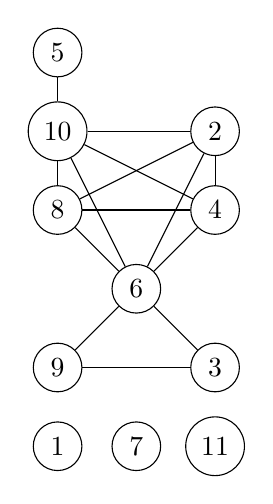
\begin{tikzpicture}
\node[shape=circle,draw=black] (A) at (0,5) {5};
\node[shape=circle,draw=black] (B) at (0,4) {10};
\node[shape=circle,draw=black] (C) at (2,4) {2};
\node[shape=circle,draw=black] (D) at (0,3) {8};
\node[shape=circle,draw=black] (E) at (2,3) {4};
\node[shape=circle,draw=black] (F) at (1,2) {6};
\node[shape=circle,draw=black] (G) at (0,1) {9};
\node[shape=circle,draw=black] (H) at (2,1) {3};
\node[shape=circle,draw=black] (I) at (0,0) {1};
\node[shape=circle,draw=black] (I) at (1,0) {7};
\node[shape=circle,draw=black] (I) at (2,0) {11};
\path [] (A) edge node[left] {} (B);
\path [] (B) edge node[left] {} (C);
\path [] (B) edge node[left] {} (D);
\path [] (B) edge node[left] {} (E);
\path [] (B) edge node[left] {} (F);
\path [] (C) edge node[left] {} (D);
\path [] (C) edge node[left] {} (E);
\path [] (C) edge node[left] {} (F);
\path [] (D) edge node[left] {} (E);
\path [] (D) edge node[left] {} (F);
\path [] (E) edge node[left] {} (F);
\path [] (F) edge node[left] {} (G);
\path [] (F) edge node[left] {} (H);
\path [] (G) edge node[left] {} (H);
\end{tikzpicture}
\end{align*}

The blocks are: $V(5, 10) $, $V(6,9,3)$, $V(1)$, $V(7)$, $V(11)$, $V(10,2,4,6,8)$
\end{question}

\begin{question}{5}
	Give a formula for the number of spanning trees of G in terms of the number of spanning trees of its blocks.	\\
	$\tau(G) = \sum{\tau(\text{Blocks})}$
\end{question}

\begin{question}{6}
\end{question}

\begin{question}{7}
\end{question}

\begin{question}{8}
\end{question}

\begin{question}{9}
\end{question}

\begin{question}{10}
\end{question}


% --------------------------------------------------------------
%     You don't have to mess with anything below this line.
% --------------------------------------------------------------

\end{document}
